\section{617 --- Merge Two Binary Trees}
Given two binary trees and imagine that when you put one of them to cover the other, some nodes of the two trees are overlapped while the others are not.

You need to merge them into a new binary tree. The merge rule is that if two nodes overlap, then sum node values up as the new value of the merged node. Otherwise, the NOT null node will be used as the node of new tree.

\paragraph{Example 1:}

\begin{flushleft}
\textbf{Input}:

\begin{figure}[H]
\begin{tikzpicture}
[every node/.style={draw, circle, fill=gray!20!, minimum size=5mm}]
\node(1){1}
child{node{3} child{node{5}} child[missing]}
child{node{2}};

\node[right= of 1, xshift=4cm ]{2}
child{node{1} child[missing] child{node{4}}}
child{node{3} child[missing] child{node{7}}};
\end{tikzpicture}
\end{figure}


\textbf{Output}:

\begin{figure}[H]
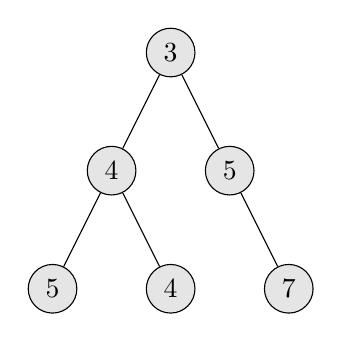
\begin{tikzpicture}
[every node/.style={draw, circle, fill=gray!20!, minimum size=5mm}]
\node{3}
child{node{4} child{node{5}} child{node{4}}}
child{node{5} child[missing] child{node{7}}};
\end{tikzpicture}
\end{figure}


\end{flushleft}

\paragraph{Note:} 
\begin{itemize}
\item The merging process must start from the root nodes of both trees.
\end{itemize}

\subsection{Recursion}
We can traverse both the given trees in a \textbf{preorder} fashion. 
\begin{itemize}
    \item At every step, we check if the current node is not null for both the trees. If so, we add the values in the current nodes of both the trees and update the value in the current node of the first tree to reflect this sum obtained. 
    \item At every step, we also call the original function with the left children and then with the right children of the current nodes of the two trees. If at any step, one of these children happens to be null, we return the child of the other tree(representing the corresponding child subtree) to be added as a child subtree to the calling parent node in the first tree. 
    \item At the end, the first tree will represent the required resultant merged binary tree.
\end{itemize}